\section{Практическая часть}
\subsection{Постановка задачи}

Для обеспечения работы ООО <<Цветочная лавка>> необходимо дать возможность одновременной работы двум разным типам пользователей - Оператору и Клиенту.

Для Оператора критично иметь возможность:
\begin{itemize}
	\item Создавать, изменять и удалять букеты
	\item Создавать, изменять и удалять типы букетов
	\item Создавать, изменять и удалять фото букетов
	\item Создавать, изменять и удалять цвета букетов
	\item Создавать, изменять и удалять цветы
	\item Создавать, изменять и удалять подарки
	\item Создавать, изменять и удалять категории подарков
	\item Создавать, изменять и удалять фотографии подарков
	\item Создавать, изменять и удалять промокоды
	\item Вести отслеживание заказов
\end{itemize}

Для Клиента необходимо предоставить возможность:
\begin{itemize}
	\item Ознакомиться с перечнем доступных букетов и подарков
	\item Добавить позиции в корзину
	\item Произвести заказ 
\end{itemize}

\subsection{Проектирование базы данных}

Список таблиц, которые нам потребуются:

\begin{itemize}
	\item Букеты
	\item Заказы
	\item Клиенты
	\item Корзины пользователей
	\item Подарки
	\item Промокоды
	\item Типы подарков
	\item Типы букетов
	\item Фотографии букетов
	\item Фотографии подарков
	\item Цветы
	\item Ценовая категория
	\item Элементы корзины пользователей	
\end{itemize}

\begin{table}[!h]
	\centering
	\caption{Букеты}
	\begin{tabular}{|c|c|}
		\hline
		Поле & Тип поля \\ \hline
		Идентификатор & UUID \\ \hline
		Название & Строка \\ \hline
		Описание & Текст \\ \hline
		Цена & Целое число \\ \hline
		Ширина & Целое число \\ \hline
		Высота & Целое число \\ \hline
		Вес & Целое число \\ \hline
	\end{tabular}
\end{table}

\begin{table}[!h]
	\centering
	\caption{Фотографии букетов}
	\begin{tabular}{|c|c|}
		\hline
		Поле & Тип поля \\ \hline
		Идентификатор & UUID \\ \hline
		Путь к файлу & Строка \\ \hline
	\end{tabular}
\end{table}

\begin{table}[!h]
	\centering
	\caption{Типы букетов}
	\begin{tabular}{|c|c|}
		\hline
		Поле & Тип поля \\ \hline
		Идентификатор & UUID \\ \hline
		Тип букета & Строка \\ \hline
	\end{tabular}
\end{table}

\begin{table}[!h]
	\centering
	\caption{Ценовая категория}
	\begin{tabular}{|c|c|}
		\hline
		Поле & Тип поля \\ \hline
		Идентификатор & UUID \\ \hline
		Цена от & Целое число \\ \hline
		Цена до & Целое число \\ \hline		
	\end{tabular}
\end{table}

\begin{table}[!h]
	\centering
	\caption{Заказ}
	\begin{tabular}{|c|c|}
		\hline
		Поле & Тип поля \\ \hline
		Идентификатор & UUID \\ \hline
		Статус & Целое число \\ \hline
		Оплачено & Логический тип \\ \hline
		Дата доставки & Дата \\ \hline
		Адрес доставки & Строка \\ \hline
	\end{tabular}
\end{table}


\subsection{Проектирование приложения}

Список страниц, который нам потребуется с точки зрения клиента:

\begin{itemize}
	\item Список товаров
	\item Страница товара
	\item Страница корзины
	\item Страница оформления заказа
\end{itemize}

\begin{figure}[H]
	\centering
	\caption{Список товаров}
	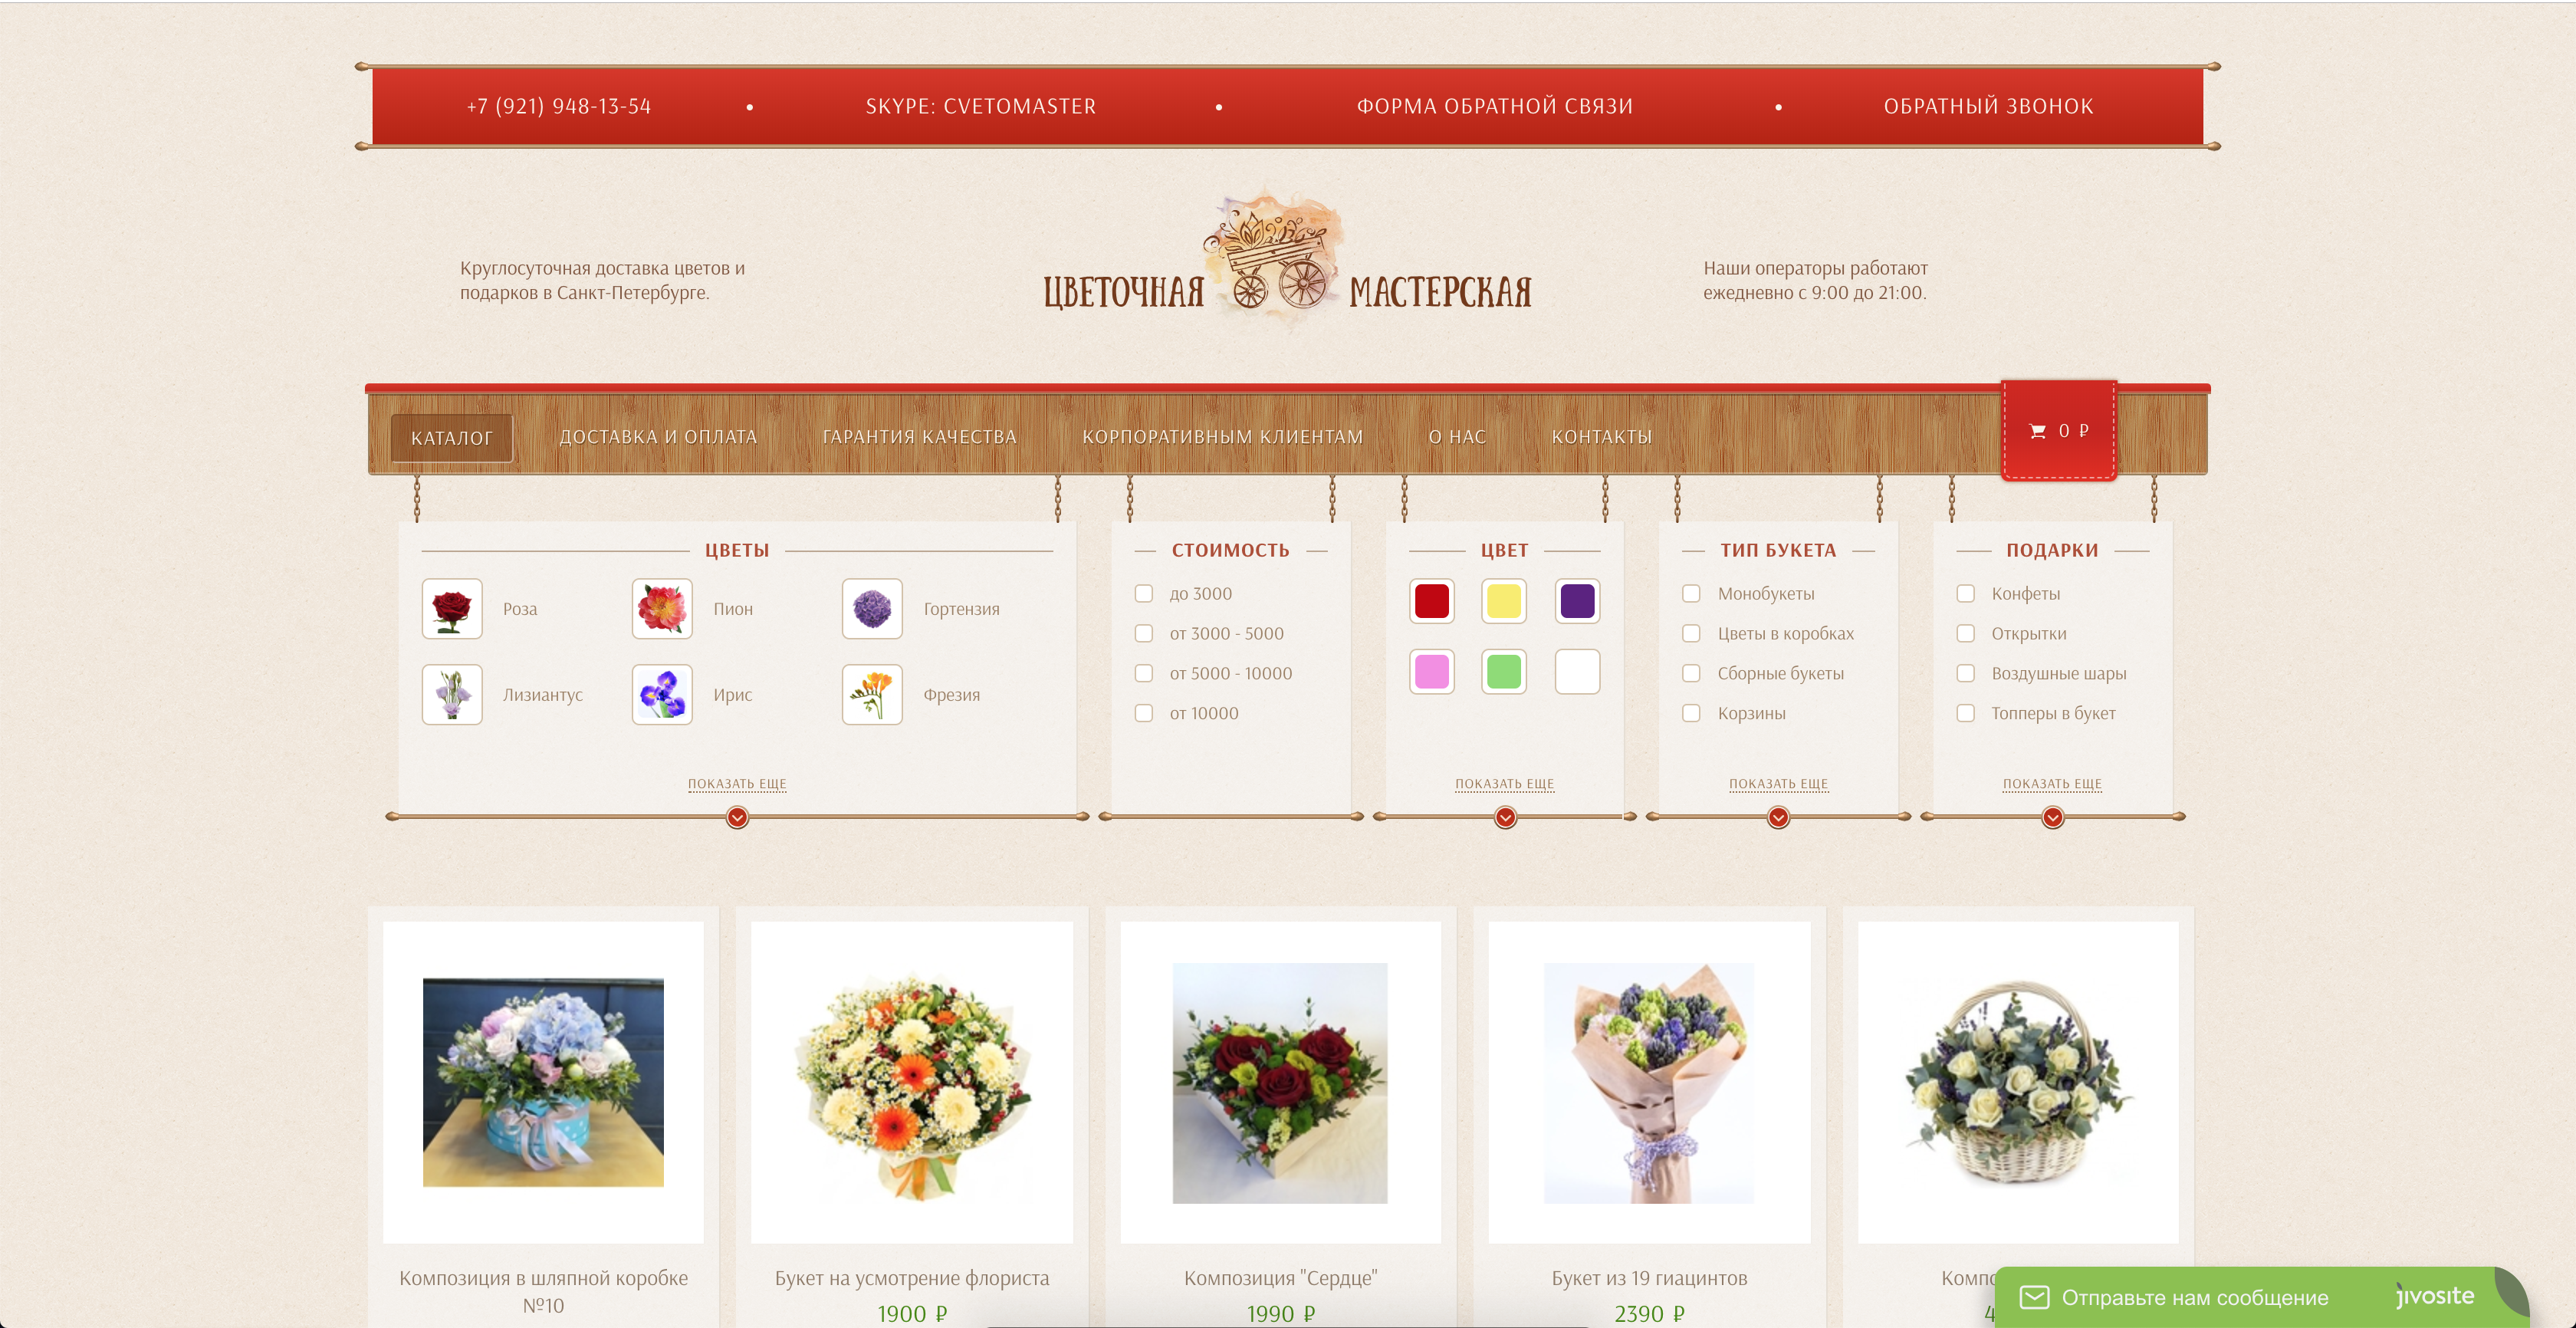
\includegraphics[width=.9\textwidth]{img/1.png}
\end{figure}

\begin{figure}[H]
	\centering
	\caption{Страница товара}
	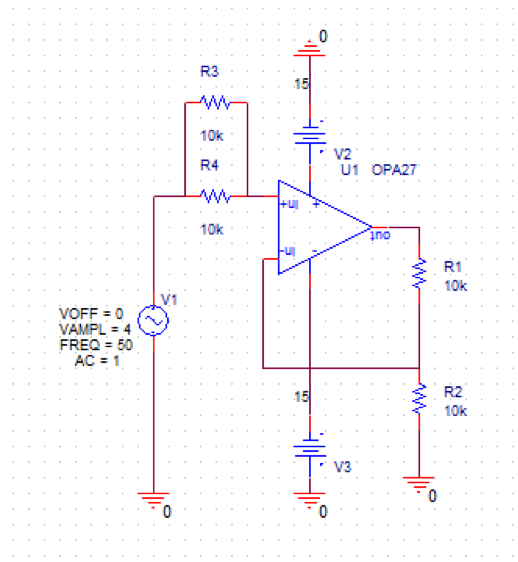
\includegraphics[width=.9\textwidth]{img/2.png}
\end{figure}

\begin{figure}[H]
	\centering
	\caption{Страница корзины}
	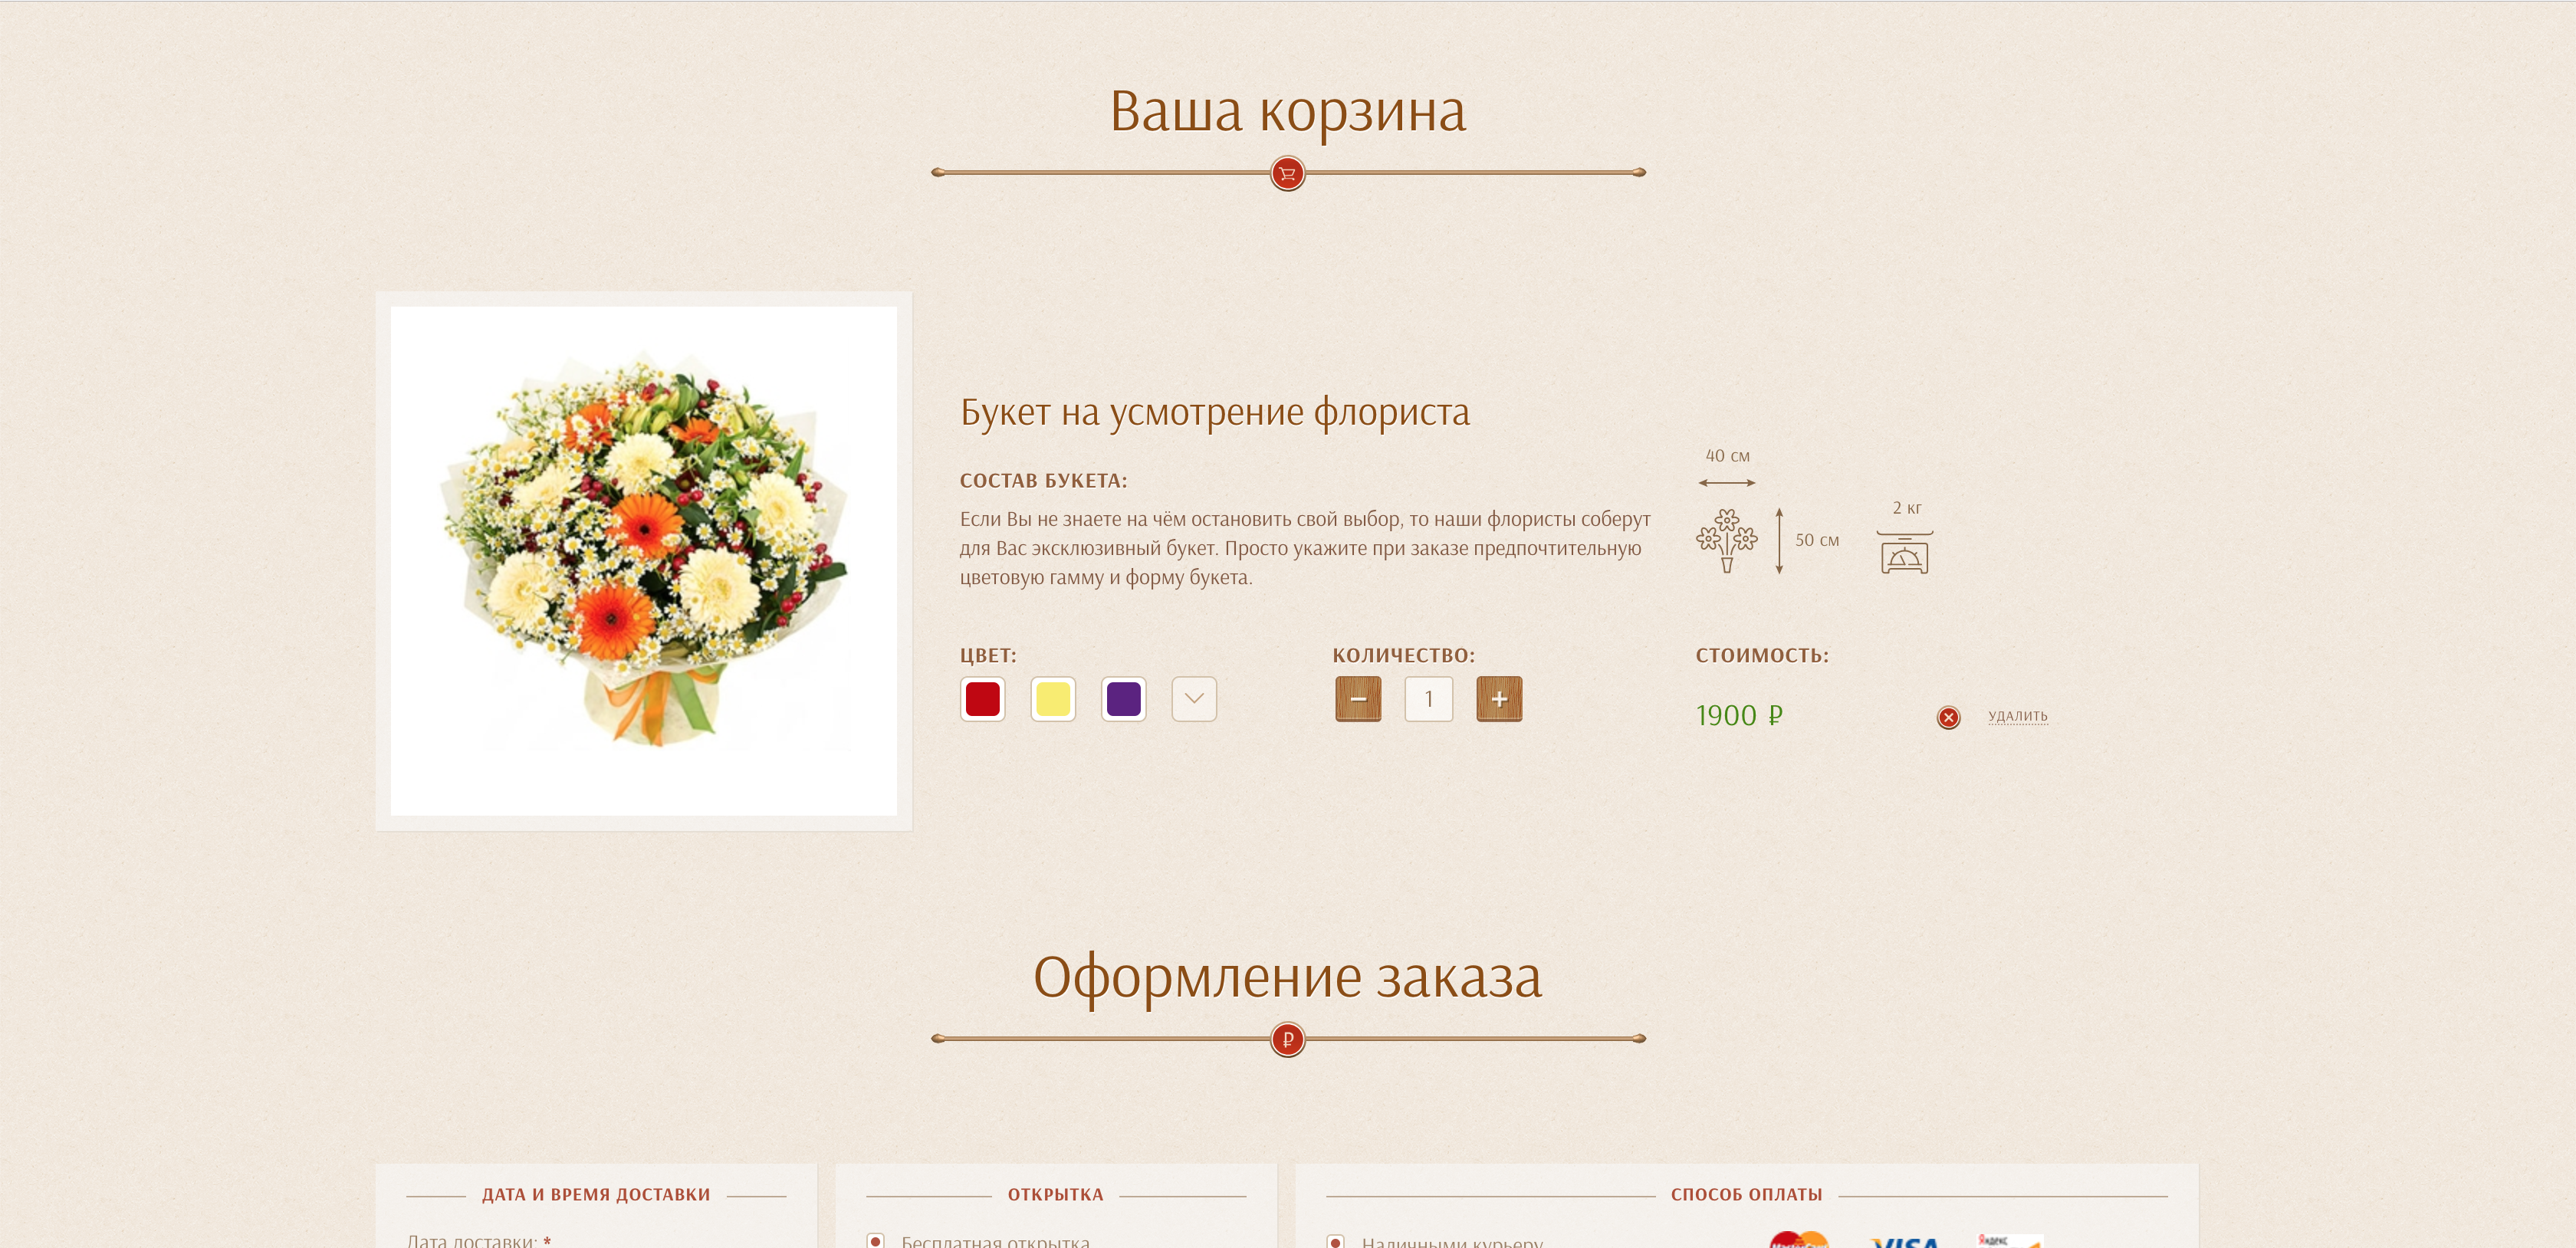
\includegraphics[width=.9\textwidth]{img/3.png}
\end{figure}

\begin{figure}[H]
	\centering
	\caption{Страница оформления заказа}
	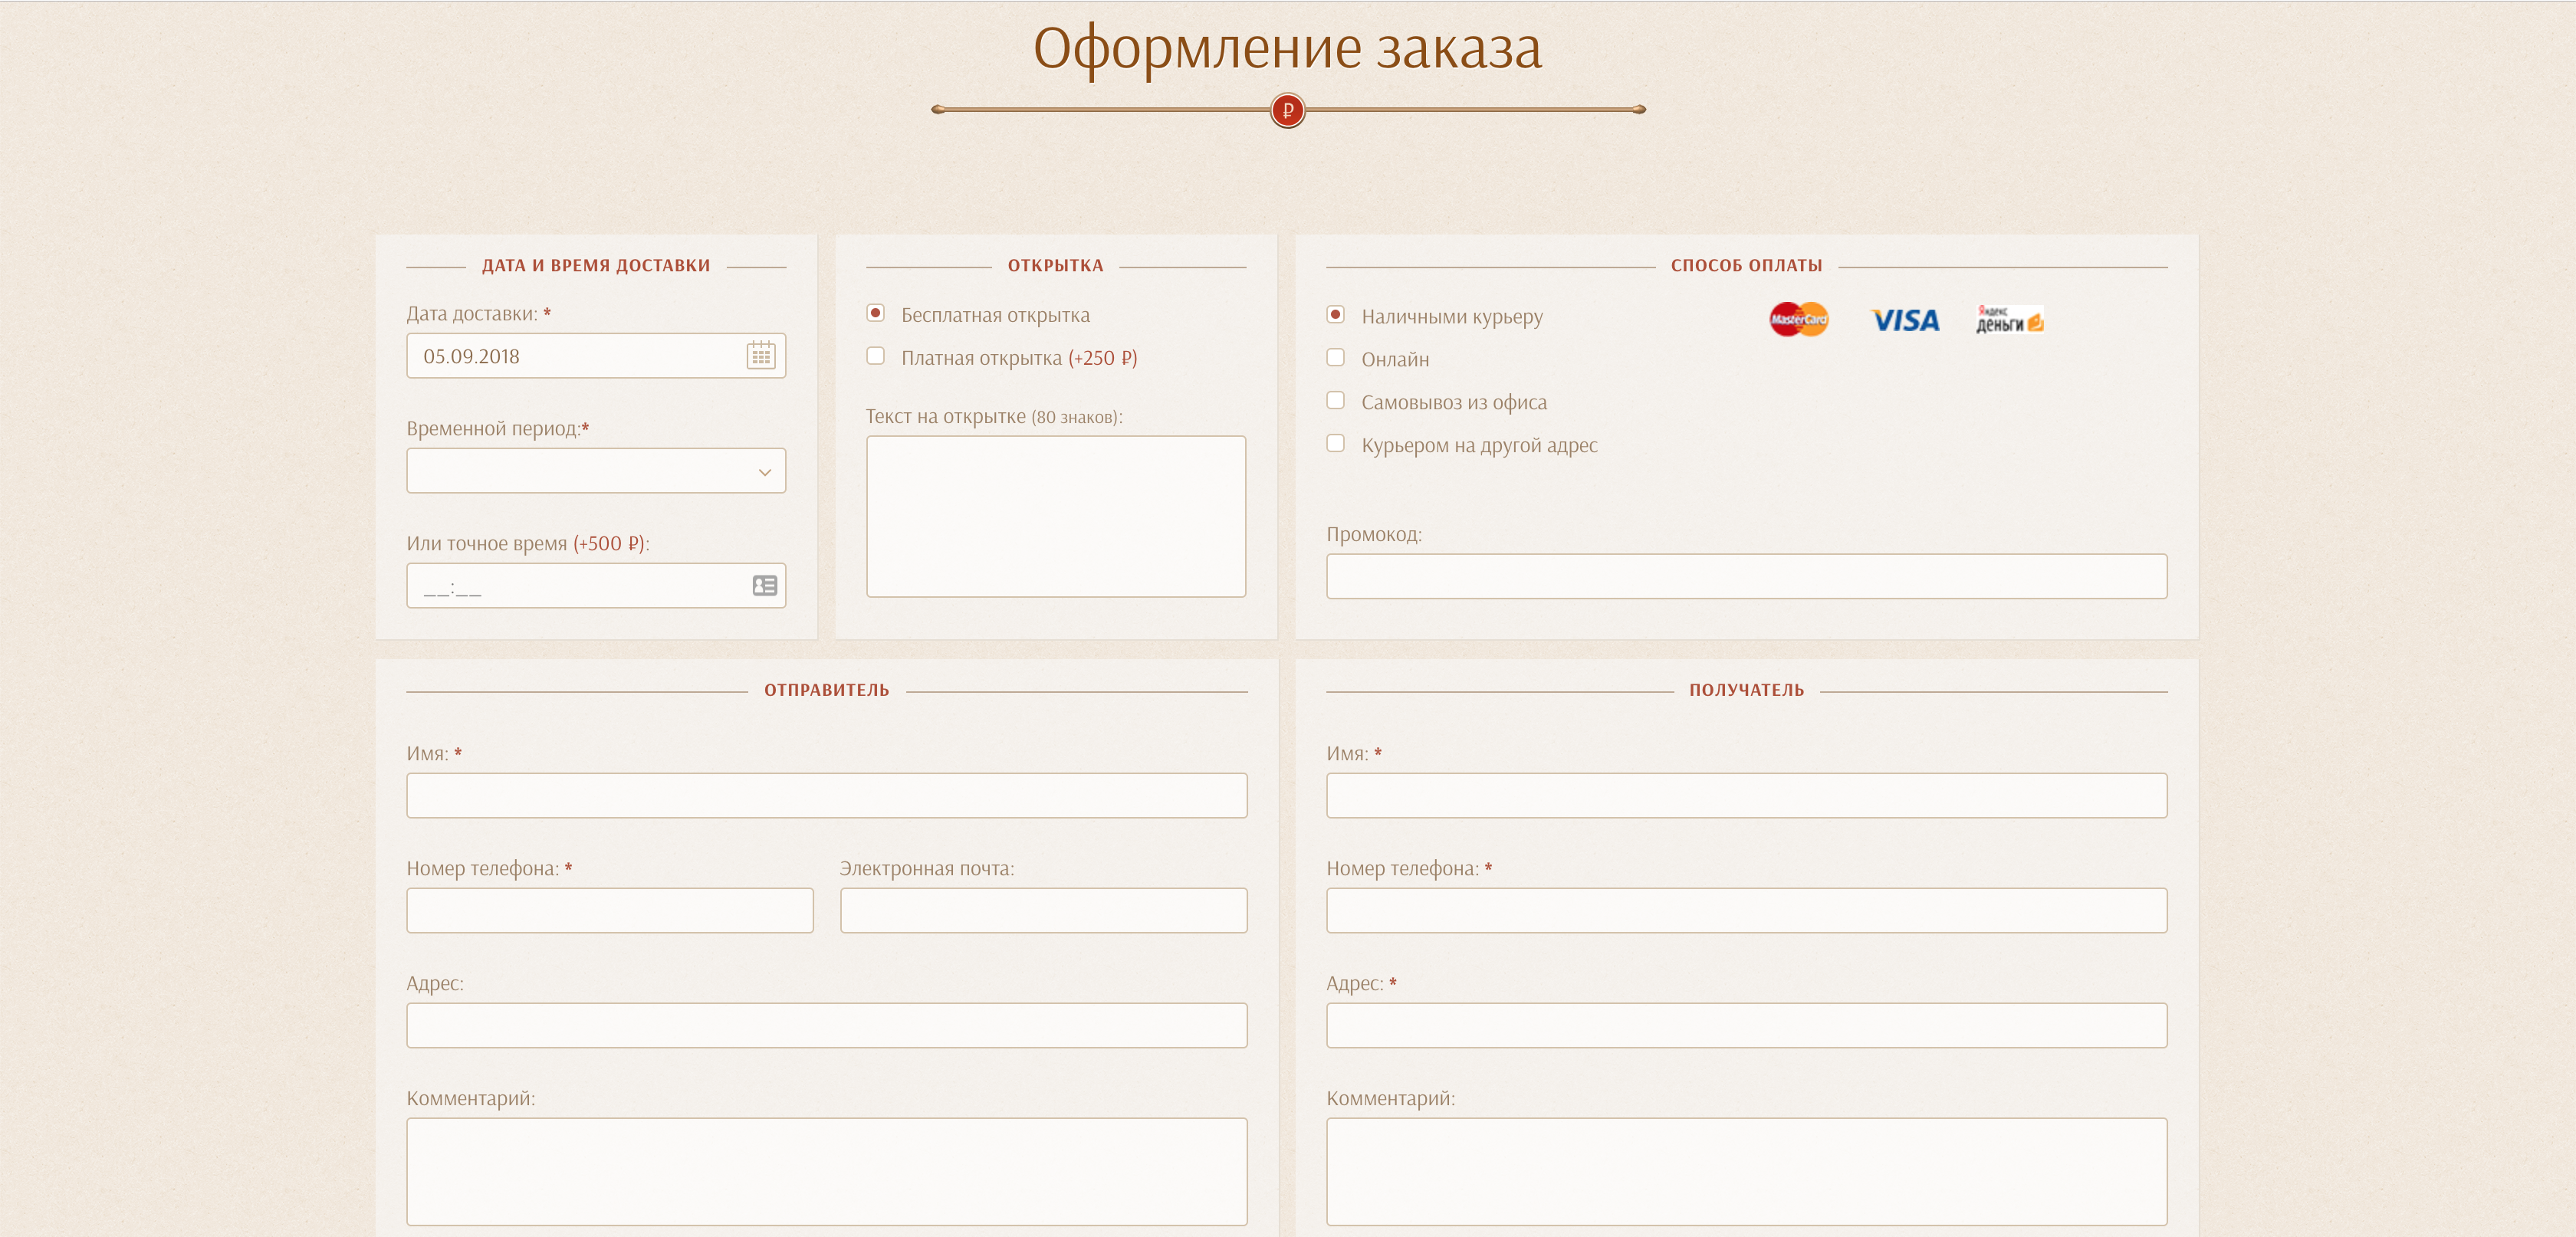
\includegraphics[width=.9\textwidth]{img/4.png}
\end{figure}


Список страниц, который нам потребуется с точки зрения оператора:

\begin{itemize}
	\item Управление товарами
	\item Управление заказами
\end{itemize}

\begin{figure}[H]
	\centering
	\caption{Административная часть сайта}
	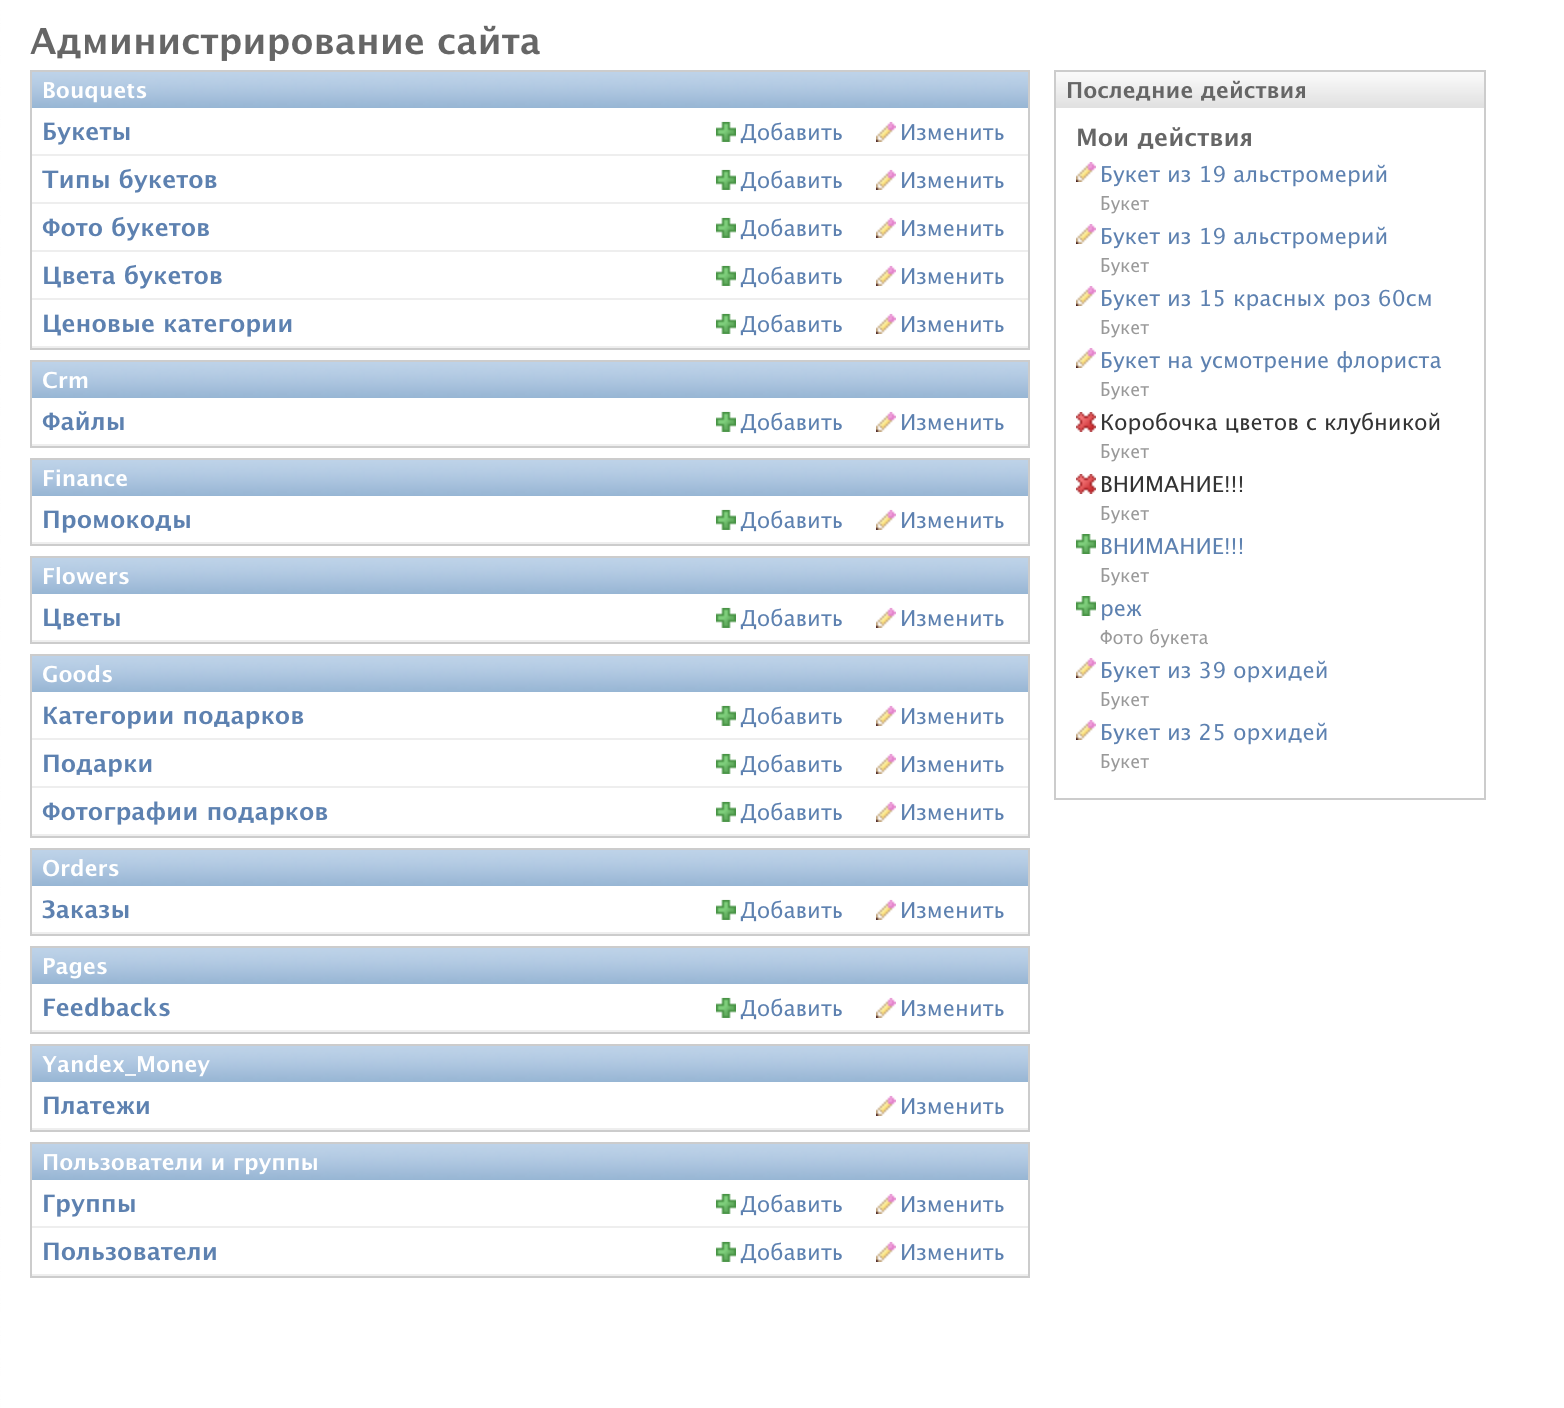
\includegraphics[width=.9\textwidth]{img/5.png}
\end{figure}


\subsection{Программа и методика испытаний}

\begin{table}[H]
		\begin{tabular}{|l|p{7cm}|p{7cm}|}
			\hline
			№ & Действие & Результат \\ \hline
			1 & \multicolumn{2}{p{9cm}|}{Сценарий <<Клиент заказывает цветы на сайте>>} \\ \hline
			1.1 & Зайти на сайт & На сайте открывается каталог цветов \\ \hline
			1.2 & Нажать на букет & Открывается страница выбранного букета \\ \hline
			1.3 & Добавить товар в корзину & Сумма в корзине увеличивается на стоимость товара \\ \hline
			1.4 & Перейти в корзину & Открывается страница корзины, на которой доступен полный перечень товаров и общая стоимость заказа \\ \hline
			1.5 & Заполнить поля и подтвердить заказ & На сайте открывается каталог цветов \\ \hline
			2 & \multicolumn{2}{p{9cm}|}{Сценарий <<Администратор наполняет каталог>>} \\ \hline
			2.1 & Зайти в административную часть сайта & Открывается административная часть сайта \\ \hline
			2.2 & Открыть каталог и нажать на "Добавить букет" & Открывается форма создания букета \\ \hline
			2.3 & Заполнить поля и нажать "Сохранить" & Новый букет сохраняется и появляется в административной части и в каталоге на сайте \\ \hline									
		\end{tabular}
\end{table}


\subsection{Протокол испытаний}

\begin{table}[H]
	\begin{tabular}{|l|p{5cm}|p{3cm}|p{3cm}|p{3cm}|}
		\hline
		№ & Шаг испытаний (проверок) & № пункта
методики
 & Отметка о прохождении (да/нет) & Примечания \\ \hline
		1 & Зайти на сайт & 1.1 & Да & \\ \hline
		2 & Нажать на букет & 1.2 & Да & \\ \hline
		3 & Добавить товар в корзину & 1.3 & Да & \\ \hline
		4 & Перейти в корзину & 1.4 & Да & \\ \hline
		5 & Заполнить поля и подтвердить заказ & 1.5 & Да & \\ \hline
		6 & Зайти в административную часть сайта & 2.1 & Да & \\ \hline
		7 & Открыть каталог и нажать на "Добавить букет" & 2.2 & Да & \\ \hline
		8 & Заполнить поля и нажать "Сохранить" & 2.3 & Да & \\ \hline
	\end{tabular}
\end{table}